\chapter{Definitions}

TODO we shall introduce a number of definitions, some only auxiliary, some necessary in the whole work

\section{XML Tree}

We shall use the representation introduced in \cite{fidax}, where an XML file is represented by a labeled tree consisting of nodes for elements, attributes and simple text data. This tree shall be called an \textit{XML tree}. For a given node $v$ of an XML tree we define $label(v)$ (name of the node in in the document, only for elements and attributes), $id(v)$ (unique identifier across the document) and $value(v)$ (text content, only for attributes and simple text data) in the same way as the referenced article does.

Without a loss of generality we ignore the actual ordering of nodes in the tree.

\paragraph{Example}

This example introduces an XML file fragment that will be used for demonstration throughout this work. XML tree representing it is in Figure \ref{image-definitions-example-xml-tree}, where each node is annotated with a triple $label(v) : id(v) : value(v)$.

\begin{verbatim}
<x>
  <y a="1" b="2"/>
  <y a="3" c="4"/>
  <y/>
  <z a="1"/>
</x>
\end{verbatim}

\begin{figure}
  \caption{Example XML Tree}
  \label{image-definitions-example-xml-tree}
  \centering
    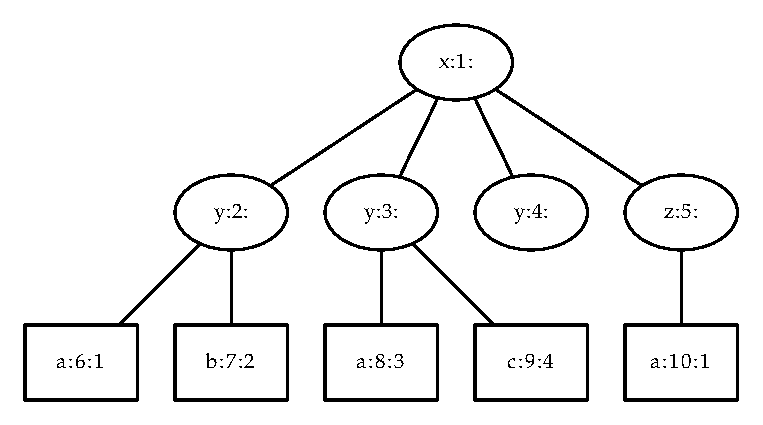
\includegraphics[width=\textwidth]{images/definitions/xml-tree}
\end{figure}

Furthermore, we denote $I$ % TODO fix the capital I
the set of all ids and $V$ % TODO fix the capital V
the set of all values in the document. We will need two more definitions from the article.

\begin{define}[Node equality]
	$v_1$ and $v_2$ are node equal, written $v_1 =_n v_2$ iff $id(v_1) = id(v_2)$.
\end{define}

\begin{define}[Value equality]
	$v_1$ and $v_2$ are value equal, written $v_1 =_v v_2$ iff $value(v_1) = value(v_2)$.
\end{define}

\section{ID, IDREF, IDREFS Attributes}

According to \cite{Bray:08:EML}, an XML attribute may have the type \textit{ID}, \textit{IDREF} or \textit{IDREFS} (among others). Following constraints are related to these types.

\begin{quote}
\textbf{Validity constraint: ID}

Values of type \textbf{ID} \textsc{must} match the Name production. A name \textsc{must not} appear more than once in an XML document as a value of this type; i.e., \textbf{ID} values \textsc{must} uniquely identify the elements which bear them.

\textbf{Validity constraint: One ID per Element Type}

An element type \textsc{must not} have more than one \textbf{ID} attribute specified.

\textbf{Validity constraint: ID Attribute Default}

An \textbf{ID} attribute \textsc{must} have a declared default of \textbf{\#IMPLIED} or \textbf{\#REQUIRED}.

\textbf{Validity constraint: IDREF}

Values of type \textbf{IDREF} \textsc{must} match the Name production, and values of type \textbf{IDREFS} \textsc{must} match Names; each Name \textsc{must} match the value of an \textbf{ID} attribute on some element in the XML document; i.e. \textbf{IDREF} values \textsc{must} match the value of some ID attribute.
\end{quote}

\section{XML Keys}

TODO

\subsection{According to Specification}

TODO compare them to ID attributes

\subsection{According to \cite{keX}}

TODO show how a XML key is defined using the keX notation % this is a terrible sentence

\section{Attribute Mappings}

Now we return to \cite{fidax} to define the notion of an \textit{attribute mapping} (or AM for short). \nomenclature{AM}{Attribute Mapping}
We will use a different definition (without introducing keys from \cite{keX} for now) that will however give us the same result.

\begin{define}[$\Sigma^E$, $\Sigma^A$, $\Sigma$]
	$\Sigma^E$ is the set of all element labels, $\Sigma^A$ is the set of all attribute labels. $\Sigma = \Sigma^E \cup \Sigma^A$ is their union and effectively the set of all labels in the document (simple text data nodes do not have a label).
\end{define}

\begin{define}[Attribute mapping]
	For $x \in \Sigma^E$ and $y \in \Sigma^A$ we define the attribute mapping of y over x, denoted $M_{x}^{y}$, the $I \times I$ % TODO fix the capital I
	relation defined by
	\[M_{x}^{y} = \{ (z,w): label(z) = x, label(w) = y, parent(w) = z \}\]
\end{define}

Thus the relation $M_{x}^{y}$ contains edges in the XML tree connecting element nodes labeled $x$ and attribute nodes labeled $y$.

TODO more from the article?

\paragraph{Example}
The XML tree from Figure \ref{image-definitions-example-xml-tree} has the following non-empty AMs: $M_{y}^{a} = \{(2,6), (3,8)\}$, $M_{y}^{b} = \{(2,7)\}$, $M_{y}^{c} = \{(3,9)\}$ and $M_{z}^{a} = \{(5,10)\}$.

\subsection{Attribute Mapping Model}

TODO

\section{ID Set}

TODO

\section{Attribute Mapping Weight}

TODO

\subsection{Support}

TODO

\subsection{Coverage}

TODO